\chapter{Scene Analysis and the ANASS Framework}
\label{ch:scene}

Before selecting or tuning a denoising algorithm, \projectshort{} characterizes each benchmark scenario through \emph{full-dimensional signal analysis}. For every scene, three aligned signals are studied: clean speech ($s$), isolated noise ($d$, obtained as $\mathrm{mix}-s$), and the noisy mixture ($y=s+d$). The resulting statistics are stored in \texttt{analysis/scene\_details/*\_metrics.json}, summarized in Markdown reports under \texttt{analysis/reports/}, and aggregated into global ANASS parameter guidance in \texttt{analysis/anass\_init\_ranges.json}. This chapter describes the analysis methodology, key findings, and the Adaptive Noise Adaptive Spectral Subtraction (ANASS) design framework that translates measurements into algorithm parameters.

\section{Full-Dimensional Signal Analysis}
\label{sec:full_dim_analysis}

\subsection{Analysis Pipeline}

The analysis pipeline computes descriptors in four domains for each of the 15 benchmark scenes (\chapref{ch:system}):

\begin{enumerate}
  \item \textbf{Time domain} --- global mean, variance, peak amplitude, RMS, dynamic range; frame-wise short-time energy and zero-crossing rate (ZCR); voiced/unvoiced/noise autocorrelation structure.
  \item \textbf{Frequency domain} --- Welch power spectral density (PSD); band-wise SNR in low (0--300\,Hz), mid (300--3400\,Hz), and high (3400--8000\,Hz) bands; spectral flatness and normalized spectral entropy; clean-speech formant/harmonic peaks.
  \item \textbf{Time--frequency domain} --- STFT spectrograms; local SNR maps and histograms; non-stationarity index; spectral flux; temporal and spectral correlation decay.
  \item \textbf{Statistical domain} --- amplitude and power distribution goodness-of-fit (Kolmogorov--Smirnov tests); baseline fixed-parameter spectral-subtraction residual statistics (RMS, kurtosis, flatness) as a defect predictor.
\end{enumerate}

Together, these domains expose not only global SNR level but also \emph{where} and \emph{when} speech is masked---information that a single scalar SNR cannot capture.

\subsection{Time-Domain Characteristics}

Short-time RMS energy distinguishes speech-dominated frames (high variance, wide dynamic range) from noise-dominated frames. ZCR complements energy: voiced speech exhibits moderate ZCR with strong periodic autocorrelation peaks (e.g., lag 96 samples at 16\,kHz), whereas broadband noise approaches ZCR${}\approx 0.5$ with weak autocorrelation.

Table~\ref{tab:time_domain_compare} contrasts two white-noise scenes at different global SNR levels. At 15\,dB (scene01), noise RMS is low and energy-based separability between clean and noise frames remains high ($d=0.99$). At 5\,dB (scene02), noise energy approaches speech energy in many frames ($d=0.24$), making energy-only voice activity unreliable---a direct motivation for multi-feature soft gating in ANASS Module~1.

\begin{table}[H]
  \centering
  \caption{Time-domain separability for white-noise scenes (Cohen's $d$, clean vs.\ noise frames).}
  \label{tab:time_domain_compare}
  \begin{tabular}{lccc}
    \toprule
    \textbf{Feature} & \textbf{scene01 (15\,dB)} & \textbf{scene02 (5\,dB)} & \textbf{Interpretation} \\
    \midrule
    Short-time energy & 0.985 & 0.241 & Energy gating weakens at low SNR \\
    Zero-crossing rate  & 2.097 & 2.063 & ZCR remains discriminative \\
    Spectral flatness   & 1.750 & 1.755 & Flatness robust across SNR \\
    \bottomrule
  \end{tabular}
\end{table}

\subsection{Frequency-Domain Characteristics}

Band-wise SNR reveals strong inter-band imbalance even when global SNR appears moderate. For scene01 at 15\,dB global SNR, high-band SNR is only 1.46\,dB while mid-band SNR reaches 18.83\,dB. For scene02 at 5\,dB, the high band falls to $-8.50$\,dB. Such imbalance motivates frequency-dependent over-subtraction ($\alpha_{\mathrm{low}}$ vs.\ $\alpha_{\mathrm{high}}$) in ANASS Module~2.

Spectral flatness further separates speech (harmonic, low flatness; median $\approx 0.006$ for clean) from noise (near-flat; mean $\approx 0.56$ for white noise). In the mixture, flatness shifts toward noise-like values in low-SNR frames, providing a useful VAD auxiliary feature.

\subsection{Time--Frequency Characteristics}

Local SNR is computed per STFT bin and summarized by distribution statistics. Scene01 exhibits a median local SNR of $-14.2$\,dB with 76.7\% of bins below 0\,dB despite 15\,dB global SNR---demonstrating that \emph{global SNR overestimates} local intelligibility. Scene02 is more extreme: 89.7\% of bins fall below 0\,dB and the median local SNR is $-24.1$\,dB.

\begin{figure}[H]
  \centering
  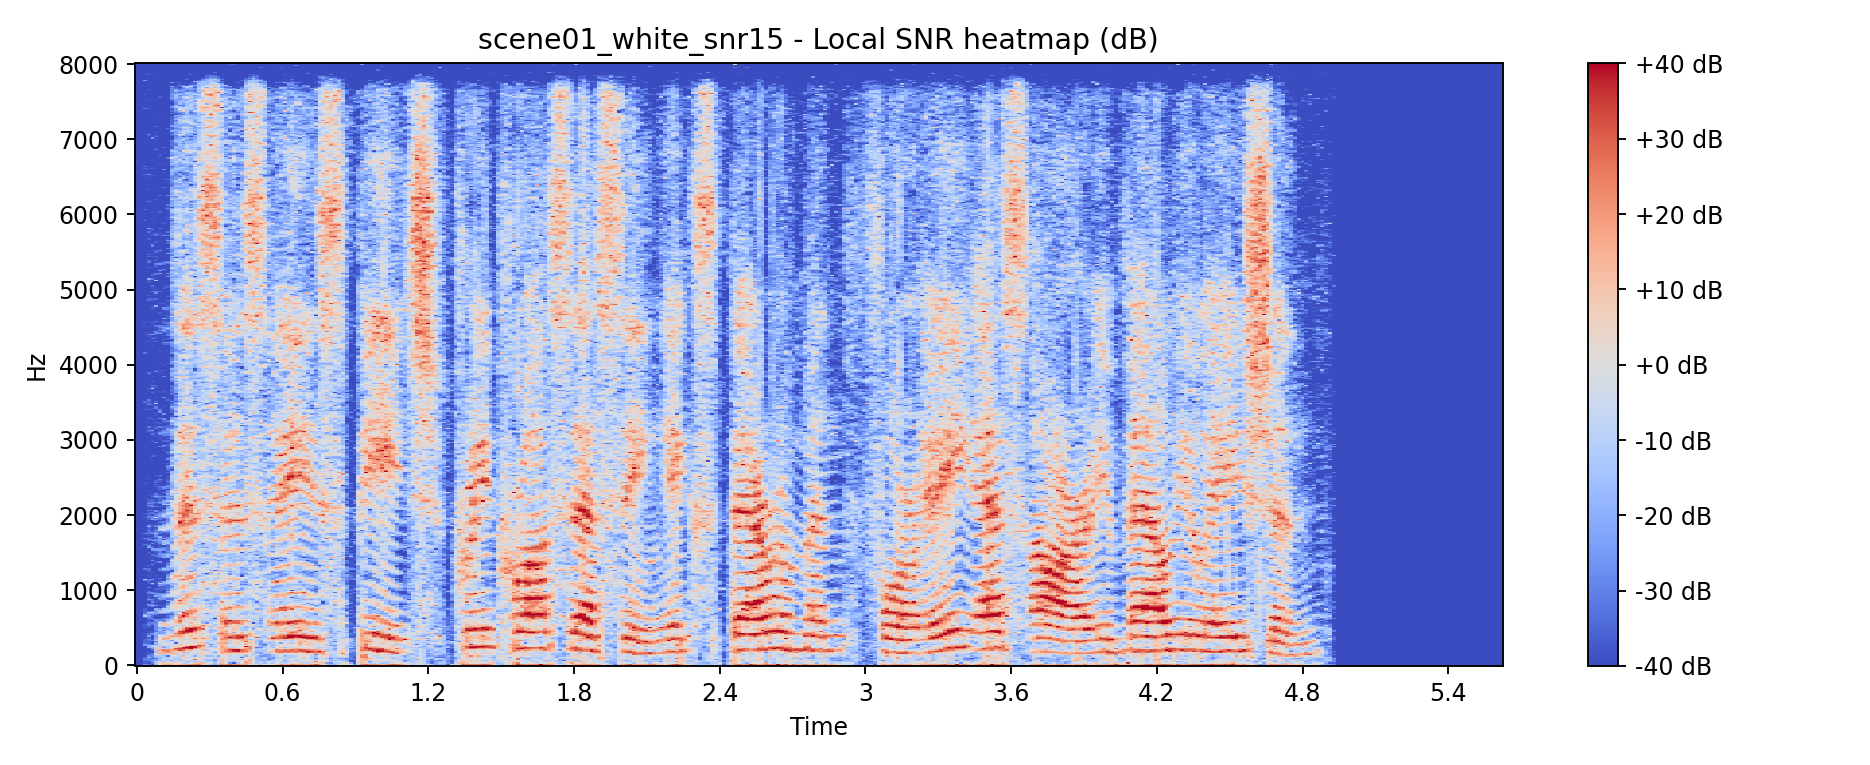
\includegraphics[width=0.6\textwidth]{../analysis/priority_plots/scene01_white_snr15_local_snr_heatmap.png}
  \caption{Local SNR heatmap for \texttt{scene01\_white\_snr15}. Large low-SNR regions explain why fixed spectral subtraction fails.}
  \label{fig:local_snr_heatmap}
\end{figure}

\begin{figure}[H]
  \centering
  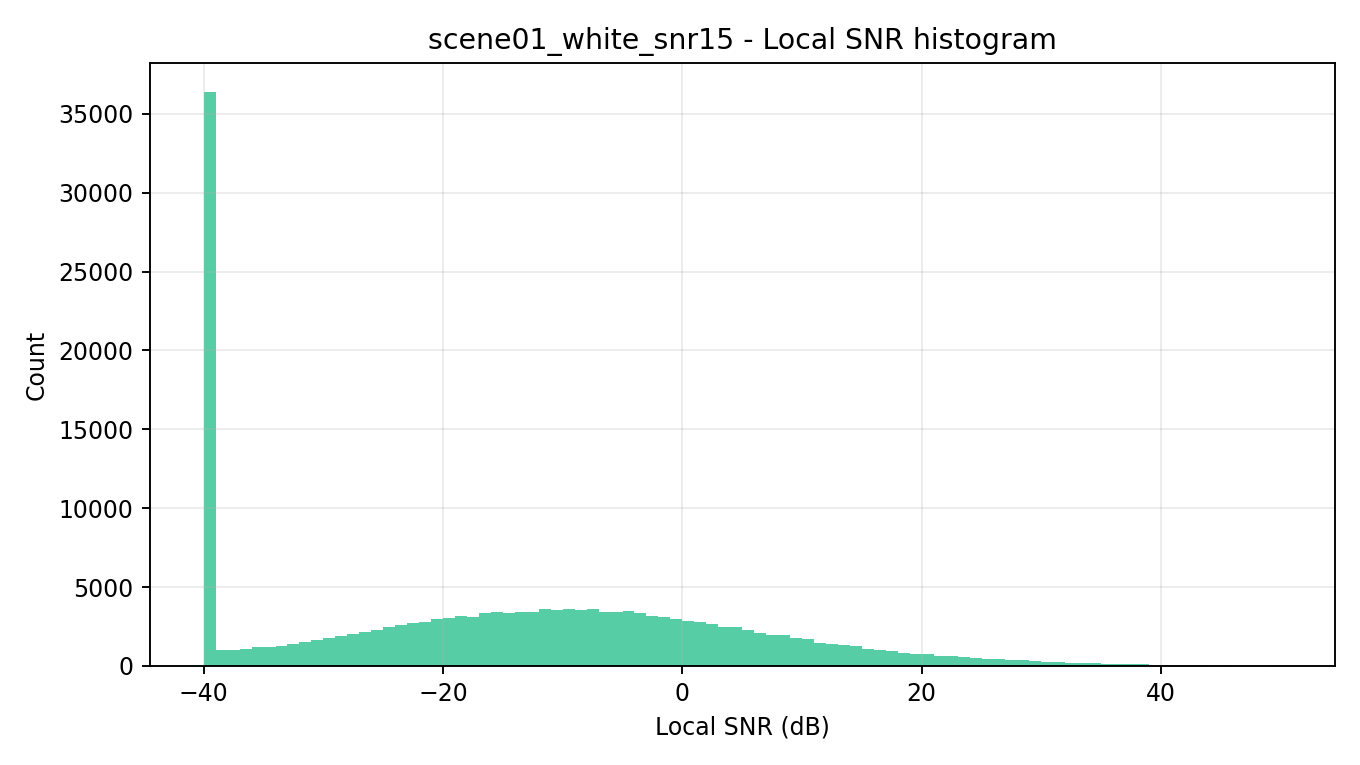
\includegraphics[width=0.6\textwidth]{../analysis/priority_plots/scene01_white_snr15_local_snr_hist.png}
  \caption{Local SNR histogram for scene01. The heavy left tail drives adaptive rather than fixed suppression.}
  \label{fig:local_snr_hist}
\end{figure}

Non-stationarity indices near 0.81--0.83 across white-noise scenes indicate that noise statistics drift over time, supporting recursive noise trackers (MCRA) rather than a single noise profile estimated from the first frames alone.

\section{Feature Separability and Noise Typing}
\label{sec:separability}

\subsection{Cohen's $d$ Effect Sizes}

For each scene, Cohen's $d$ quantifies separability between clean-speech and noise frames in the short-time feature space:
\begin{equation}
  d = \frac{\mu_{\mathrm{clean}} - \mu_{\mathrm{noise}}}
         {\sqrt{(s_{\mathrm{clean}}^2 + s_{\mathrm{noise}}^2)/2}}.
\end{equation}
Values $|d| > 0.8$ indicate large effect sizes. Across the benchmark:

\begin{itemize}
  \item \textbf{ZCR} consistently achieves $|d| > 2$ for broadband noise, making it a reliable VAD auxiliary even when energy $d$ collapses at low SNR.
  \item \textbf{Spectral flatness} maintains $|d| \approx 1.7$ for white/pink scenes, separating harmonic speech from flat noise.
  \item \textbf{Energy} varies widely ($d=0.24$--$0.99$), confirming that energy-only gates are insufficient alone.
\end{itemize}

Structured interference reduces separability differently: chirp scene09 shows lower flatness separability ($d=0.71$) because narrowband energy overlaps speech harmonics, while ZCR separability also drops ($d=1.04$). Such scenes are flagged as \emph{priority optimization} targets requiring specialized modules (subspace projection, chirp notch) rather than generic OM-LSA alone.

\subsection{Automated Noise-Type Labels}

Each scene report assigns a noise-type label stored in JSON metrics, e.g.\
``near-white broadband'' (scene01--02), ``high-frequency dominated'' (scene09 chirp), ``tonal hum'' (scene05--06), or ``reverb + hiss'' (scene15). These labels feed the rule router (\chapref{ch:routing}) alongside numeric features.

\section{ANASS Design Framework}
\label{sec:anass}

ANASS (Adaptive Noise Adaptive Spectral Subtraction) is a three-module design template that maps scene statistics to denoiser parameters. It generalizes classical spectral subtraction by making noise estimation, suppression strength, and artifact control \emph{adaptive in time, frequency, and speech presence}.

\begin{definition}[ANASS Modules]
  \label{def:anass}
  \begin{enumerate}
    \item \textbf{Module 1 --- VAD-gated noise estimation:} estimate noise PSD $\hat{N}(k,t)$ using soft combinations of RMS, ZCR, and spectral flatness rather than hard thresholds.
    \item \textbf{Module 2 --- Adaptive over-subtraction:} apply band- and SNR-dependent oversubtraction factors $\alpha$ and spectral floors $\beta$.
    \item \textbf{Module 3 --- Musical-noise suppression:} reduce bin-wise random peaks via time--frequency smoothing and gain flooring with neighborhood consistency.
  \end{enumerate}
\end{definition}

\subsection{Module 1: VAD-Gated Noise Estimation}

Let $E(t)$, $Z(t)$, and $F(k,t)$ denote frame energy, ZCR, and spectral flatness. A soft speech presence weight for noise updating can be written as
\begin{equation}
  w_{\mathrm{speech}}(t) = \sigma\!\bigl(a_E E_{\mathrm{norm}}(t) + a_Z Z_{\mathrm{norm}}(t) + a_F F_{\mathrm{norm}}(t)\bigr),
  \label{eq:soft_vad}
\end{equation}
where $\sigma(\cdot)$ is a logistic function and normalized features are scaled to $[0,1]$ using scene-dependent percentiles from analysis reports. The noise PSD update rate becomes
\begin{equation}
  \alpha_n(t) = \alpha_{\min} + (1-w_{\mathrm{speech}}(t))\,(\alpha_{\max}-\alpha_{\min}),
\end{equation}
with $\alpha_{\min}, \alpha_{\max}$ drawn from the \texttt{noise\_update} range in Table~\ref{tab:anass_ranges}. Soft gating avoids misclassifying low-energy consonants as noise---a failure mode visible when energy Cohen's $d$ drops below 0.3 (scene02).

In the implemented OM-LSA/MCRA core (\chapref{ch:algorithms}), an equivalent mechanism uses speech presence probability $p_1(k,t)$ per bin rather than frame-level hard VAD.

\subsection{Module 2: Adaptive Over-Subtraction}

Classical magnitude subtraction follows \eqnref{eq:spec_sub} with scalar $\alpha$ and $\beta$. ANASS replaces scalars with band-specific pairs:
\begin{equation}
  \alpha(k) =
  \begin{cases}
    \alpha_{\mathrm{low}}  & f_k < 300\,\mathrm{Hz}, \\
    \alpha_{\mathrm{mid}}  & 300 \le f_k < 3400\,\mathrm{Hz}, \\
    \alpha_{\mathrm{high}} & f_k \ge 3400\,\mathrm{Hz},
  \end{cases}
\end{equation}
and similarly for $\beta(k)$. When high-band SNR falls below mid-band SNR by more than 10\,dB---as in scene01 and scene02---$\alpha_{\mathrm{high}}$ is pushed toward its upper range (3.2--4.0) while $\alpha_{\mathrm{low}}$ remains near 1.4--2.0 to preserve vowel formants.

Local SNR maps further suggest \emph{bin-wise} or \emph{frame-wise} modulation: bins with local SNR${}<0$\,dB receive stronger suppression; bins with local SNR${}>10$\,dB receive near-unity gain. The implemented system approximates this through OM-LSA gains and routing to specialized front-ends rather than explicit per-bin $\alpha$ tables.

\subsection{Module 3: Musical-Noise Suppression}

Fixed subtraction on scene01 yields baseline residual kurtosis $4.38$ and residual flatness 0.203---indicators of heavy-tailed, speckled musical noise. ANASS Module~3 applies:
\begin{itemize}
  \item temporal smoothing coefficient $\in [0.15, 0.35]$ on gain trajectories;
  \item spectral smoothing coefficient $\in [0.05, 0.16]$ across adjacent bins;
  \item a minimum gain floor to prevent isolated deep nulls;
  \item optional neighborhood consistency constraints (implemented in OM-LSA gain-floor blending).
\end{itemize}

High kurtosis ($>4$) in baseline residual reports triggers the upper smoothing range; tonal scenes with low residual kurtosis (e.g., chirp scene09, kurtosis $=2.0$) prioritize structured notch/subspace processing over aggressive smoothing.

\section{Parameter Guidance from Data}
\label{sec:param_guidance}

Table~\ref{tab:anass_ranges} consolidates parameter ranges recommended across all 15 scene reports. Values originate from \texttt{anass\_init\_ranges.json}, derived from pooled local-SNR statistics (median local SNR $\approx -0.62$\,dB; 10th percentile at $-40$\,dB clip) and repeated baseline-subtraction stress tests.

\begin{table}[H]
  \centering
  \caption{Suggested ANASS parameter ranges derived from full-dimensional scene analysis.}
  \label{tab:anass_ranges}
  \begin{tabular}{lcc}
    \toprule
    \textbf{Parameter} & \textbf{Range} & \textbf{Purpose} \\
    \midrule
    $\alpha_{\mathrm{low}}$  & $1.4$--$2.0$   & Speech protection (low/mid band) \\
    $\alpha_{\mathrm{high}}$ & $3.2$--$4.0$   & Stronger suppression (high band) \\
    $\beta_{\mathrm{low}}$   & $0.008$--$0.0176$ & Residual floor (low band) \\
    $\beta_{\mathrm{high}}$  & $0.045$--$0.0765$ & Residual floor (high band) \\
    noise\_update              & $0.87$--$0.93$  & Noise PSD tracking rate \\
    time\_smoothing            & $0.15$--$0.35$  & Temporal artifact reduction \\
    freq\_smoothing            & $0.05$--$0.16$  & Spectral artifact reduction \\
    \bottomrule
  \end{tabular}
\end{table}

\subsection{Representative Scene Snapshots}

Table~\ref{tab:scene_snapshots} contrasts three scenes illustrating how analysis drives different design emphases.

\begin{table}[H]
  \centering
  \caption{Representative scene metrics driving ANASS and routing decisions.}
  \label{tab:scene_snapshots}
  \small
  \begin{tabular}{lccc}
    \toprule
    \textbf{Metric} & \textbf{scene01} & \textbf{scene02} & \textbf{scene09} \\
    \midrule
    Global context      & white, 15\,dB & white, 5\,dB  & chirp, 8\,dB \\
    High-band SNR (dB)  & 1.46          & $-8.50$       & $-4.85$ \\
    Local SNR${}<0$ ratio & 76.7\%     & 89.7\%        & 16.8\% \\
    Energy Cohen's $d$  & 0.99          & 0.24          & 0.56 \\
    Baseline residual kurtosis & 4.38   & 4.57          & 2.00 \\
    ANASS emphasis      & HF $\alpha$, smoothing & strong smoothing, Kalman route & subspace + notch \\
    \bottomrule
  \end{tabular}
\end{table}

\begin{figure}[H]
  \centering
  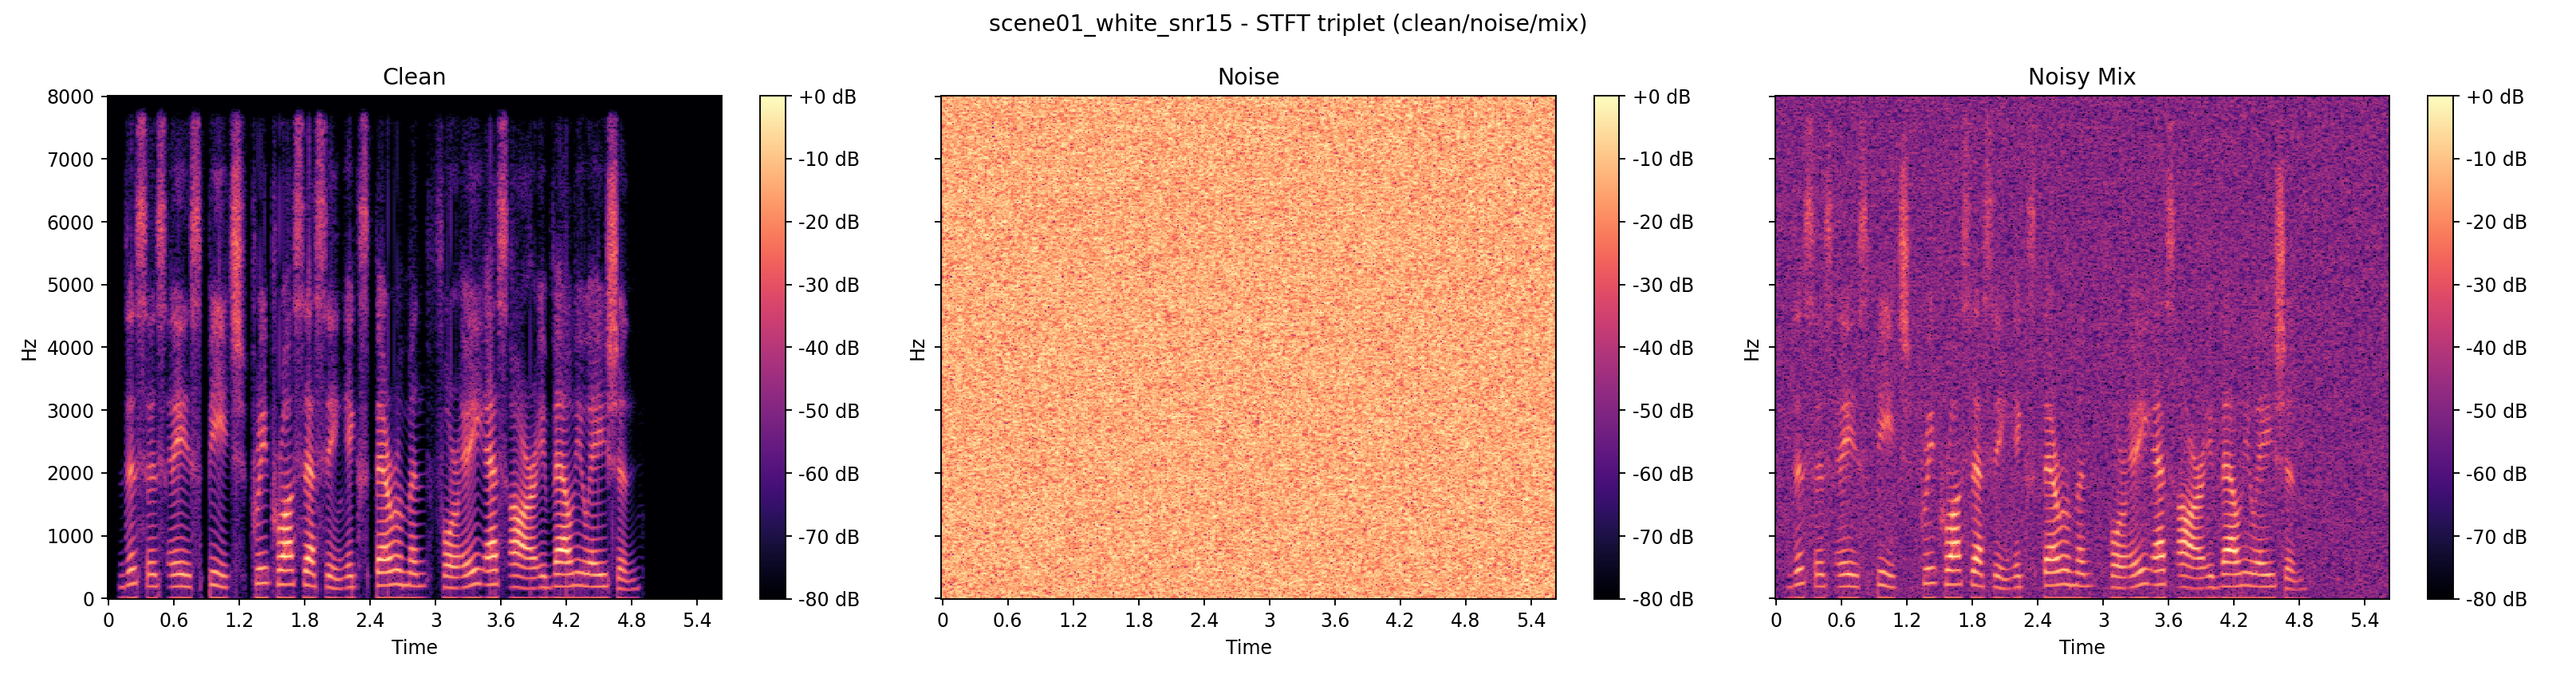
\includegraphics[width=0.92\textwidth]{../analysis/priority_plots/scene01_white_snr15_stft_triplet_clean_noise_mix.png}
  \caption{STFT triplet (clean / noise / mix) for scene01. Visual inspection confirms broadband noise masking high-frequency speech harmonics.}
  \label{fig:stft_triplet}
\end{figure}

\section{Baseline Spectral Subtraction as a Diagnostic Tool}
\label{sec:baseline_diag}

Before deploying adaptive methods, each scene report evaluates fixed-parameter spectral subtraction as a \emph{diagnostic baseline}. Residual metrics predict algorithm bottlenecks:

\begin{itemize}
  \item \textbf{High residual RMS} --- insufficient noise reduction; may need stronger $\alpha$ or specialized front-end.
  \item \textbf{High kurtosis ($>4$)} --- musical-noise risk; Module~3 smoothing required.
  \item \textbf{Elevated residual flatness} --- broadband speckle; check time--frequency smoothing and gain floors.
\end{itemize}

Scene02 baseline residual RMS (0.00805) exceeds scene01 (0.00346) by more than 2$\times$ at lower global SNR, confirming priority for low-SNR optimization and higher distillation training weights (\chapref{ch:dl}).

\section{From Analysis to Implementation}
\label{sec:analysis_to_impl}

The analysis pipeline closes the loop from measurement to deployable configuration in four steps:

\begin{enumerate}
  \item \textbf{Per-scene reports} (\texttt{analysis/reports/}) document domain-specific findings and ANASS recommendations for each WAV file.
  \item \textbf{JSON metrics} (\texttt{analysis/scene\_details/}) expose machine-readable features consumed by \texttt{router/rule\_router.py} for automatic chain selection.
  \item \textbf{Global ranges} (\texttt{anass\_init\_ranges.json}) pool statistics into default parameter intervals for OM-LSA/MCRA tuning.
  \item \textbf{Priority scenarios} flag scenes requiring specialized treatment or heavier distillation weight:
  \begin{itemize}
    \item \texttt{scene12\_babble\_like\_snr5} --- speech-like non-stationary noise;
    \item \texttt{scene10\_impulsive\_clicks\_snr9} --- impulsive outliers;
    \item \texttt{scene09\_chirp\_interference\_snr8} --- narrowband structured interference;
    \item \texttt{scene11\_intermittent\_bursts\_snr7} --- time-varying burst noise.
  \end{itemize}
\end{enumerate}

When \texttt{ratio\_lt0} (fraction of local SNR${}<0$\,dB bins) exceeds 0.75 and mid-band SNR falls below 8\,dB, the router selects \texttt{kalman\_ar} (\chapref{ch:routing}). When high-band SNR${}< -5$\,dB, subspace + OM-LSA chains are preferred. Hum and fan scenes route to adaptive notch filtering based on tonal PSD peaks and noise-type labels.

This data-driven workflow ensures that preprocessing parameters are not chosen arbitrarily: they reflect measurable speech--noise separability, local SNR geography, and predicted failure modes of classical subtraction---directly supporting the ASR preprocessing goal of presenting a cleaner, more stable front-end feature stream (\chapref{ch:introduction}).

\section{Chapter Summary}
\label{sec:scene_summary}

Full-dimensional scene analysis transforms raw noisy recordings into actionable design constraints. Cohen's $d$ separability justifies multi-feature soft VAD; band-wise and local SNR maps motivate frequency-adaptive suppression; baseline residual kurtosis motivates musical-noise control. The ANASS three-module template operationalizes these insights, and the JSON/report artifacts bind analysis to the adaptive router and algorithm library developed in subsequent chapters.
